\section{Aufgabe 1: Lennard-Jones-Fluid}

\subsection{Theorie und Vorbereitung}
In dieser Aufgabe soll ein Lennard-Jones-Fluid simuliert werden.
Dazu wird ein Ensemble von $N=n^2$ Teilchen in einem Würfel mit Kantenlänge $L=2 n \sigma$ betrachtet.
Es gelten periodische Randbedingungen, sodass die Teilchen sich bildlich gesehen in einem Torus bewegen.
Die Teilchen wechselwirken über das Lennard-Jones-Potential
\begin{equation}
    \phi(r) = 4 \epsilon \left[ \left( \frac{\sigma}{r} \right)^{12} - \left( \frac{\sigma}{r} \right)^6 \right]
\end{equation}
mit $r$ als Abstand der Teilchen und den Parametern $\epsilon$ und $\sigma$.
Die Wechselwirkung ist dabei auf den Abstand $r < \frac{L}{2}$ beschränkt.
Die Gleichung wird in Einheiten von $\sigma$ und $\epsilon$ angegeben und die Masse der Teilchen ist $m=1$.
\\
Die Bewegung der Teilchen wird durch das Newtonsche Bewegungsgesetz
\begin{equation}
    m \ddot{\vec{r}} = \vec{F}(\vec{r}) = - \nabla \phi(\vec{r})
\end{equation}
beschrieben.
Die Kraft $\vec{F}$ bzw. Beschleunigung $\ddot{\vec{r}}$ (da $m=1$) ergibt sich aus dem negativen Gradienten des Potentials $\phi$.
In diesem Fall ist die Kraft also
\begin{equation}
    \vec{F}(\vec{r}) = 24 \epsilon \left[ 2 \left( \frac{\sigma}{r} \right)^{14} - \left( \frac{\sigma}{r} \right)^8 \right] \frac{\vec{r}}{r^2} \,.
\end{equation}
wobei zu beachten ist, dass ein zusätzlicher Faktor $\frac{1}{r}$ durch die Normierung des Basisvektor $\vec{e_r} = \frac{\vec{r}}{r}$ entsteht.
\\
Die Bewegungsgleichung wird mit dem Geschwindigkeits-Verlet-Algorithmus
\begin{align}
    \vec{r}_{i+1} &= \vec{r}_i + \vec{v}_i \mathrm{d}t + \frac{1}{2} \vec{a}_i \mathrm{d}t^2 \\
    \vec{v}_{i+1} &= \vec{v}_i + \frac{1}{2} \left( \vec{a}_{i+1} + \vec{a}_{i} \right) \mathrm{d}t
\end{align}
gelöst, dabei gibt $dt$ die Zeitschrittweite an.
Wenn $n$ die Anzahl an Schritten angibt, so wird für jeden betrachteten Zeitpunkt
\begin{equation*}
    t = i \cdot \mathrm{d}t \, ,  \qquad i = 0, 1, 2, \dots, n
\end{equation*}
die Position $\vec{r}_i$ und Geschwindigkeit $\vec{v}_i$ berechnet, bis die Messzeit $T = n \cdot \mathrm{d}t$ erreicht ist.
Der Verlet-Algorithmus ist symplektisch, d.h. er erhält die Energie des Systems.
\\
Die Anfangsbedingungen werden durch eine Gitteranordnung mit Abstand $\sigma$ und zufälligen Geschwindigkeiten gewählt.
Die Geschwindigkeiten werden zuerst um den Schwerpunkt zentriert
\begin{equation}
    \vec{v}_i \rightarrow \vec{v}_i - \vec{v}_S = \vec{v}_i - \frac{1}{N} \sum_{i=1}^N \vec{v}_i
\end{equation}
Allgemein kann aus der kinetische Energie des Gesamtsystems $E_{kin}$
\begin{equation}
    E_{kin} = \frac{1}{2} \sum_{i=1}^N m_i v_i^2
\end{equation}
die Temperatur $T$ über den Zusammenhang
\begin{equation}
    T = \frac{2}{N_f k_B} E_{kin}
    \label{eq:temp}
\end{equation}
berechnet werden, wobei $N_f = 3N-3$ die Freiheitsgrade des Systems angibt.
\\
Die Anfangsgeschwindigkeiten werden skaliert, sodass die kinetische Energie der Teilchen der Temperatur $T$ entspricht.
Aus Gleichung \eqref{eq:temp} folgt unmittelbar der Skalierungsfaktor
\begin{equation}
    \alpha(t) = \sqrt{\frac{T}{T(t)}} \,.
    \label{eq:isokin}
\end{equation}
welcher auch das isokinetische Thermostat definiert.
Bei Verwendung des isokinetischen Thermostats werden die Geschwindigkeiten in jedem Zeitschritt neu skaliert, sodass die Temperatur konstant bleibt.
Ohne Thermostat werden die Geschwindigkeiten nur bei der Initialisierung skaliert.

\subsection{Äquilibrierung und Messung}
Befor die Messung der Observablen $T, E_\text{kin}, E_\text{pot}, v_S, r_{ij}$ durchgeführt werden kann, muss das System zunächst äquilibriert werden.
Das System benötigt eine gewisse Zeit, um einen stationären und physikalisch sinnvollen Zustand zu erreichen.
Die beiden Funktionen \texttt{equilibrate} und \texttt{measure} in \texttt{A1.cpp} führen die Äquilibrierung bzw. Messung durch.
Sie unterscheiden sich zum einen in der Anzahl der Zeitschritte $n_\text{equi}$ bzw. $n_\text{meas}$ und zum anderen werden keine Werte gemessen/gespeichert, wenn die Funktion \texttt{equilibrate} aufgerufen wird.
\\
Die Simulation wird vorerst ohne Thermostat für eine Anfangstemperatur $T(0)=1$ für $n=4,8,16$ durchgeführt.
Es wird die Schrittweite $dt=0.01$ verwendet und eine Messung mit $n_\text{equi}=1000$ Schritten ohne Äquilibrierung gestartet.
So können wir die Äquilibrierungszeit abschätzen.
\\
In den Abbildungen \ref{fig:obs4}($n=4$), \ref{fig:obs8}($n=8$), \ref{fig:obs16}($n=16$) sind die Energien $E$ und die Temperatur $T$ in Abhängigkeit der Zeit $t$ dargestellt.
Das System ist äquilibriert, wenn die Energien und die Temperatur konstant sind.
Folgende Äquilibrierungszeit werden den Abbildungen entnommen:
\begin{align*}
    n=4: \quad & t_\text{equi} \approx 100 \\
    n=8: \quad & t_\text{equi} \approx 100 \\
    n=16: \quad & t_\text{equi} \approx 200
\end{align*}

\begin{figure}
    \centering
    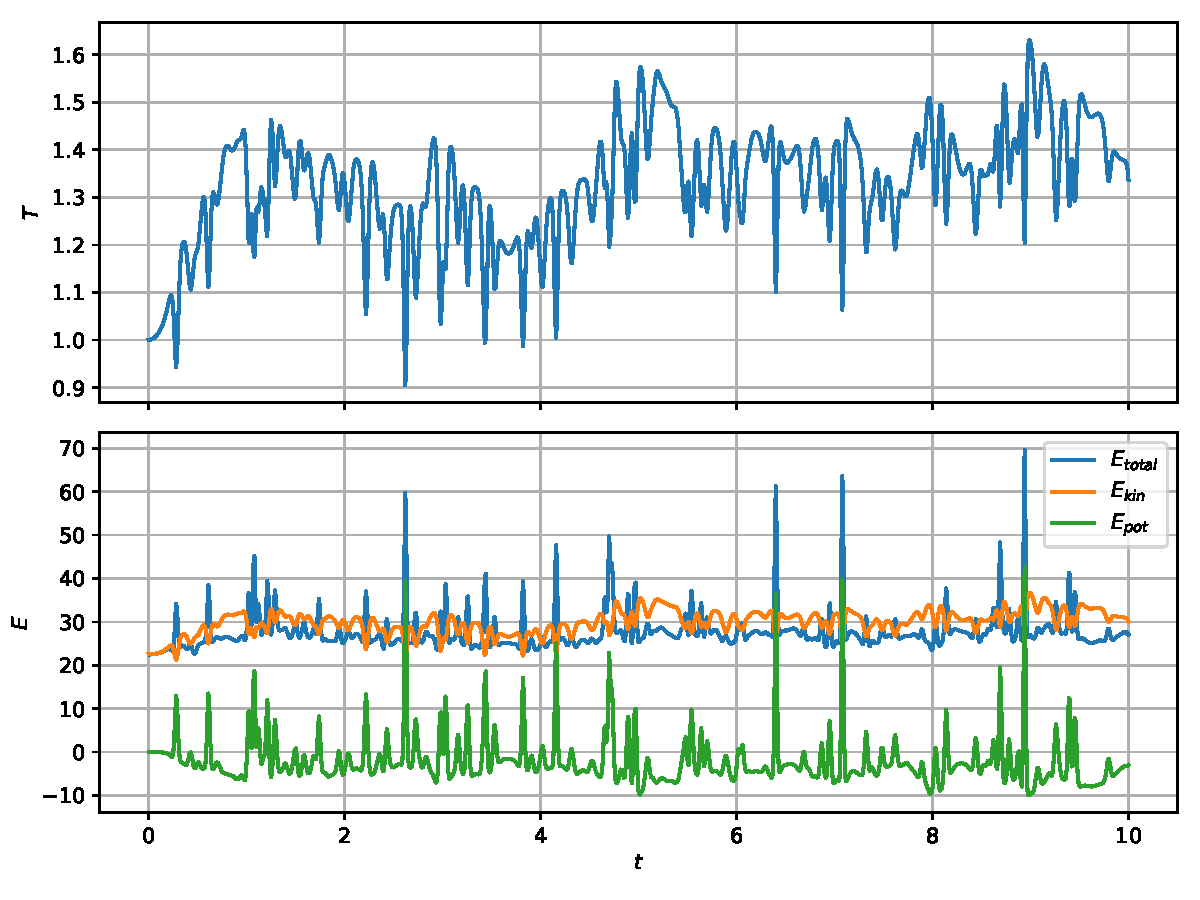
\includegraphics[width=0.8\textwidth]{content/plots/observable_n4_T1_nothermo.pdf}
    \caption{Energien und Temperatur für $n=4$ und $T(0)=1$ ohne Thermostat.}
    \label{fig:obs4}
\end{figure}
\begin{figure}
    \centering
    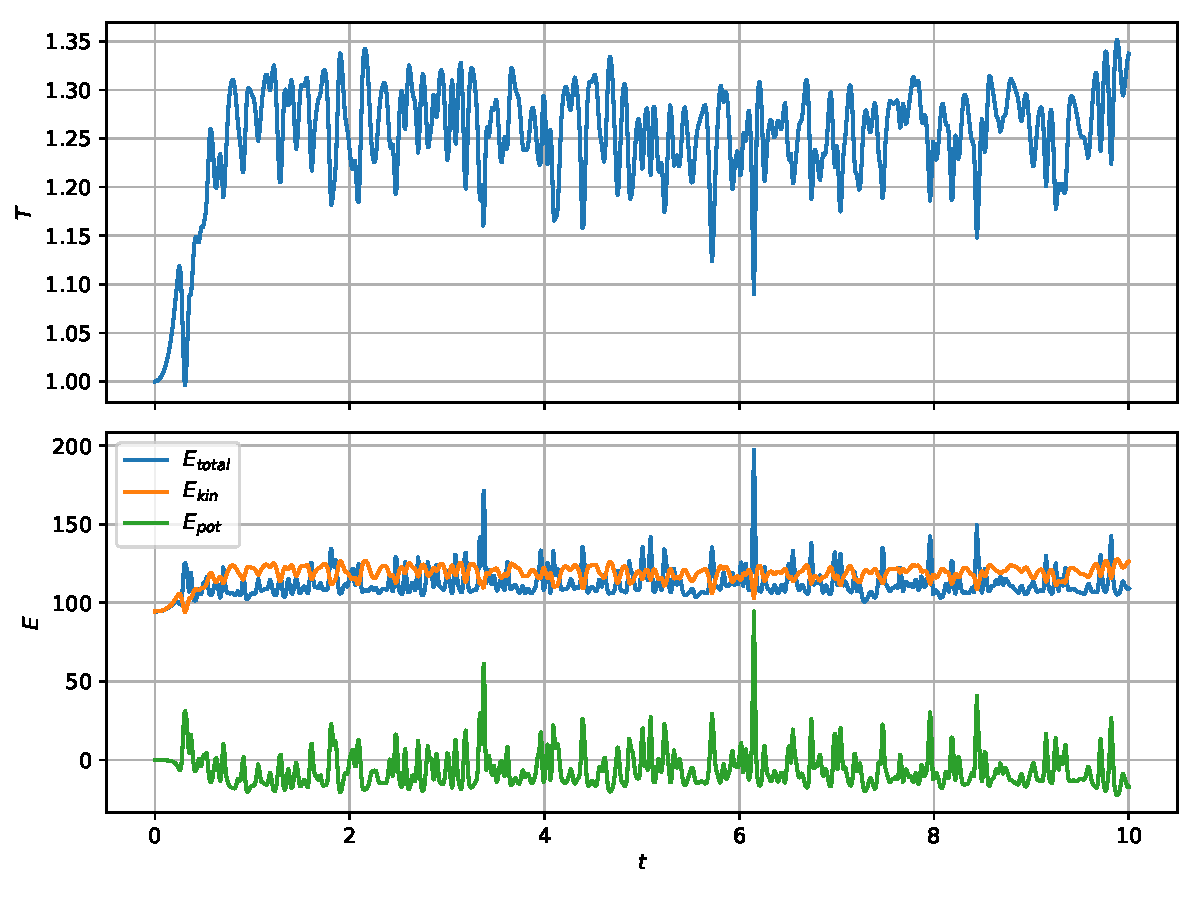
\includegraphics[width=0.8\textwidth]{content/plots/observable_n8_T1_nothermo.pdf}
    \caption{Energien und Temperatur für $n=8$ und $T(0)=1$ ohne Thermostat.}
    \label{fig:obs8}
\end{figure}
\begin{figure}
    \centering
    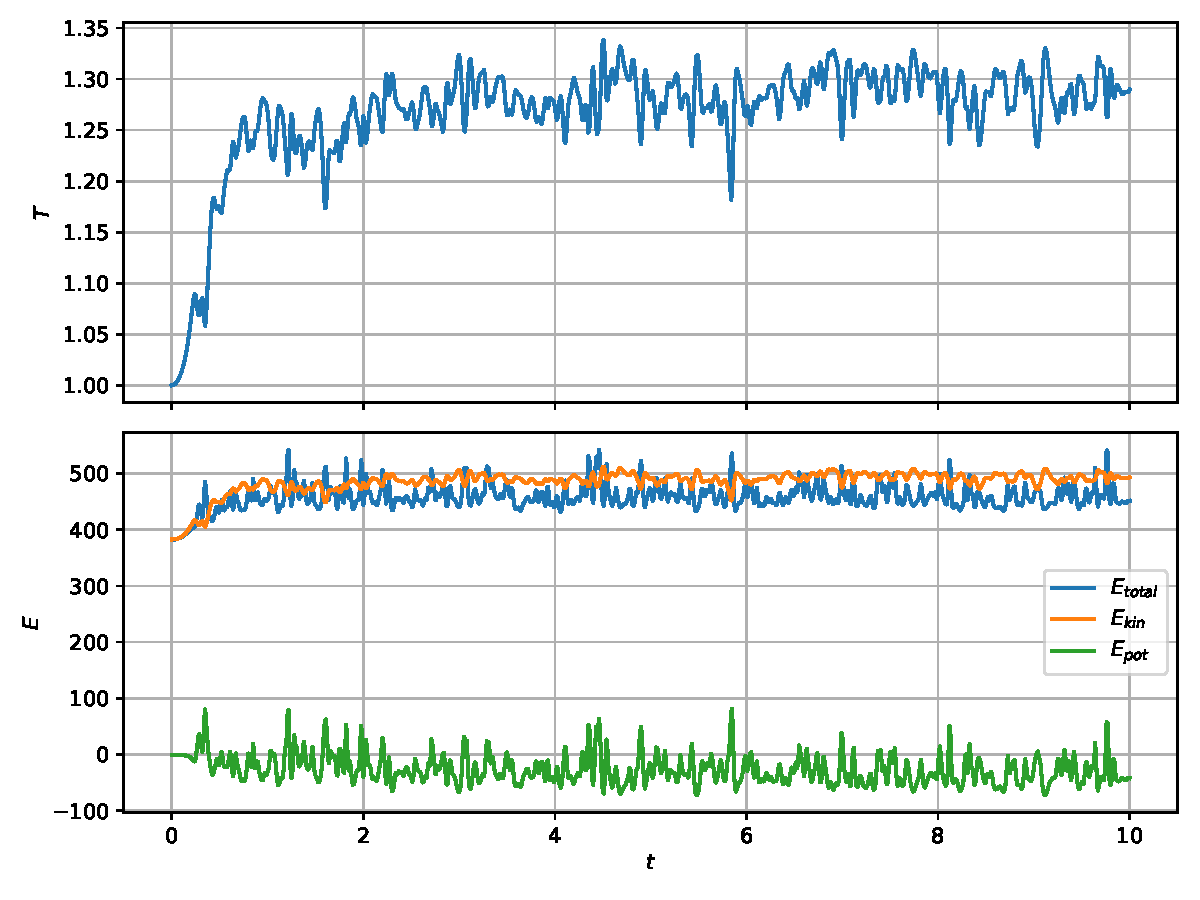
\includegraphics[width=0.8\textwidth]{content/plots/observable_n16_T1_nothermo.pdf}
    \caption{Energien und Temperatur für $n=16$ und $T(0)=1$ ohne Thermostat.}
    \label{fig:obs16}
\end{figure}
\FloatBarrier

\subsection{Paarverteilungsfunktion $g(r)$}
Die Paarverteilungsfunktion $g(r)$ gibt die Wahrscheinlichkeit an, ein Teilchen in einem Abstand $r$ zu finden.
Sie wird hier für ein gegebenes Histogramm mit $n_\text{Bins}=200$ Bins berechnet.
Das Histogramm diskretisiert die Radien $r$ von $0$ bis $L/2$.
\\
Die Funktion \texttt{calcPairCorrelation} in \texttt{A1.cpp} berechnet die Paarverteilungsfunktion aus dem Histogramm für jeden Zeitschritt.
Nach der Messung wird die Paarverteilungsfunktion über die Zeit gemittelt.
\\

Die Paarverteilung wird für ein $N=8 \cdot 8 = 64$ - Teilchensystem für drei Starttemperaturen $T=0.01, 1, 100$ untersucht.
Das System wird für $n_\text{equi}=2000$ Schritte äquilibriert und anschließend die Messung für $n_\text{meas}=10^4$ Schritte durchgeführt.
Die Schrittweite $dt=0.01$ wird für die Temperaturen $T=0.01, 1$ verwendet.
Für höhere Temperaturen wird die Schrittweite $dt=0.001$ verwendet, da das System sonst instabil wird.

%TODO
In Abbildung \ref{fig:g_001}, \ref{fig:g_1}, \ref{fig:g_100} ist die Paarverteilungsfunktion für die jeweiligen Anfangstemperaturen dargestellt.
\begin{figure}
    \centering
    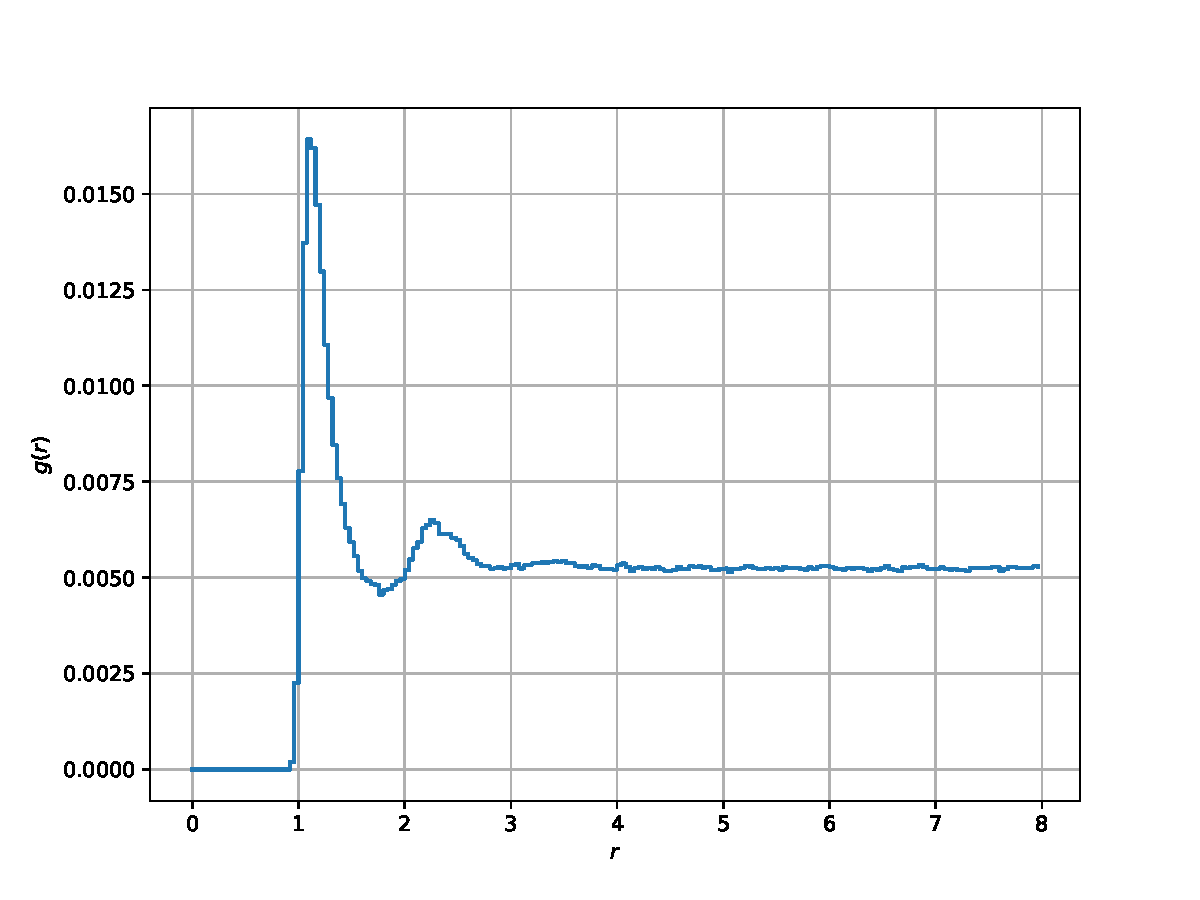
\includegraphics[width=0.8\textwidth]{content/plots/g_c)_T001.pdf}
    \caption{Paarverteilungsfunktion für $T(0)=0.01$.}
    \label{fig:g_001}
\end{figure}
\begin{figure}
    \centering
    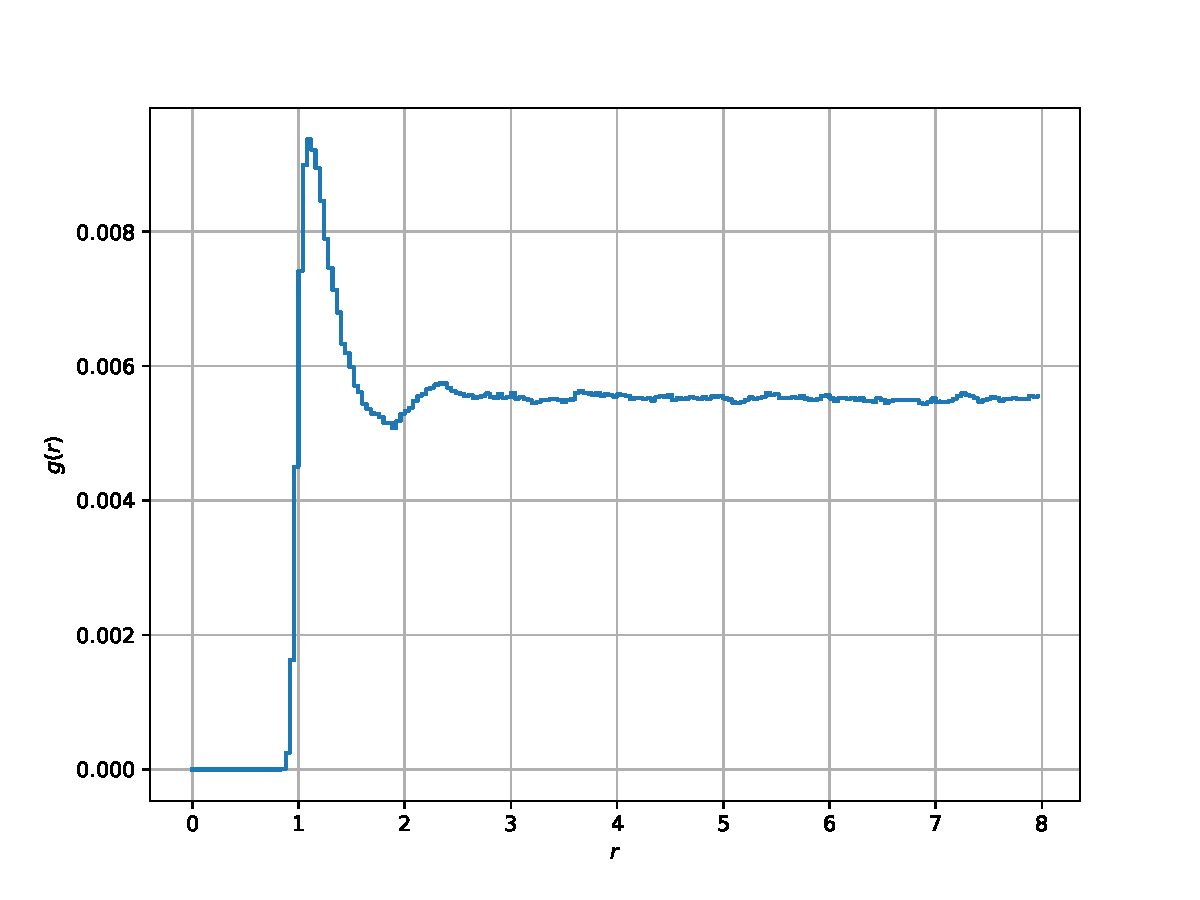
\includegraphics[width=0.8\textwidth]{content/plots/g_c)_T1.pdf}
    \caption{Paarverteilungsfunktion für $T(0)=1$.}
    \label{fig:g_1}
\end{figure}
\begin{figure}
    \centering
    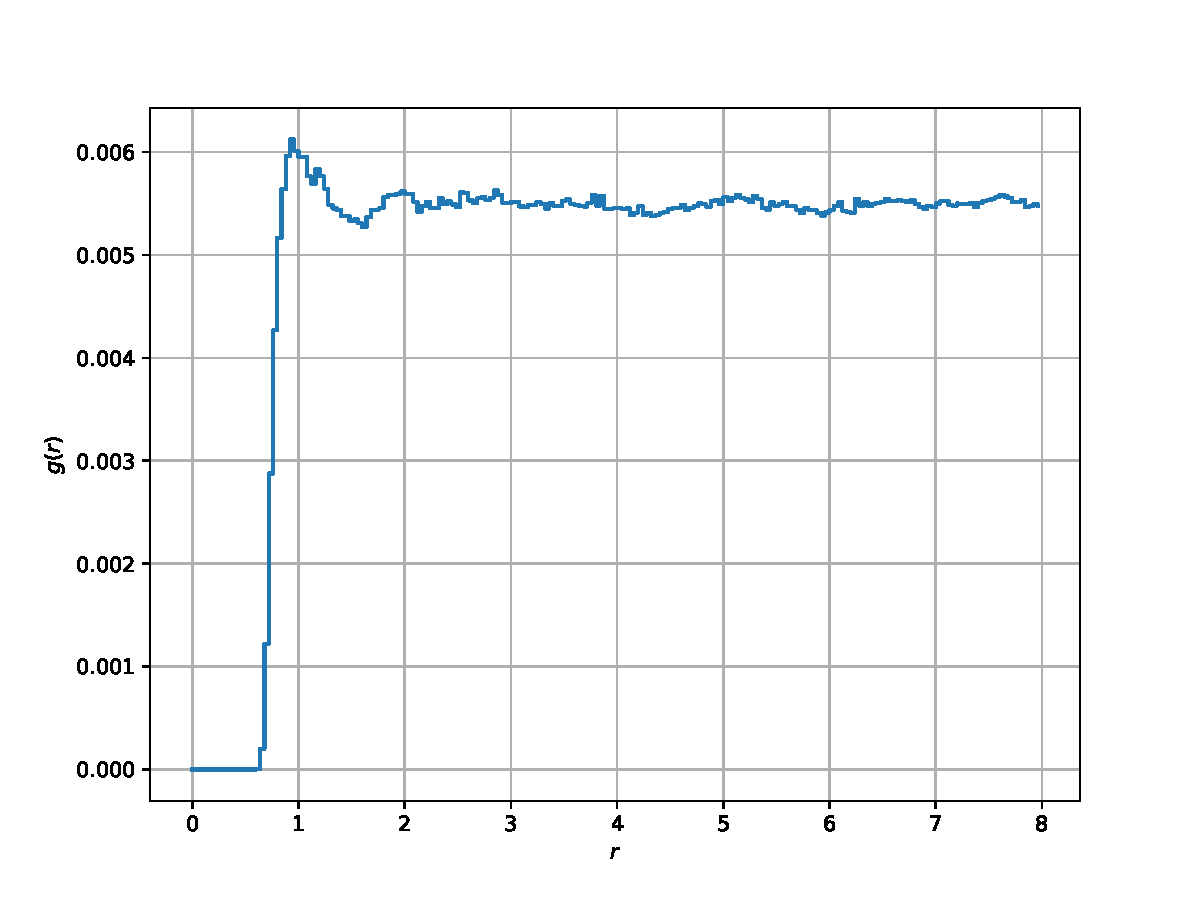
\includegraphics[width=0.8\textwidth]{content/plots/g_c)_T100.pdf}
    \caption{Paarverteilungsfunktion für $T(0)=100$.}
    \label{fig:g_100}
\end{figure}
\FloatBarrier
Die Abbildungen \ref{fig:obs_001}, \ref{fig:obs_1}, \ref{fig:obs_100} zeigen die Energien und Temperaturen in Abhängigkeit der Zeit.
\begin{figure}
    \centering
    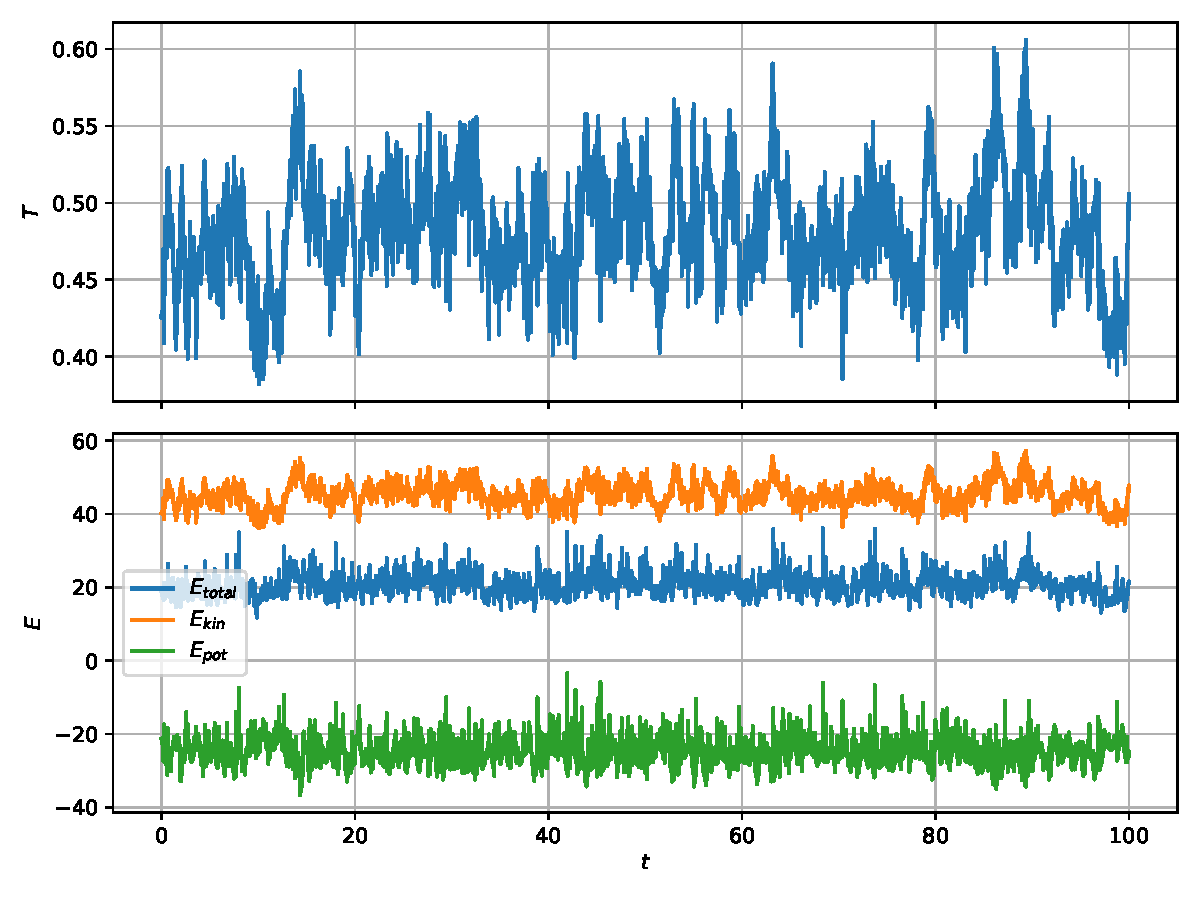
\includegraphics[width=0.8\textwidth]{content/plots/obs_c)_T001.pdf}
    \caption{Energien und Temperatur für $T(0)=0.01$.}
    \label{fig:obs_001}
\end{figure}
\begin{figure}
    \centering
    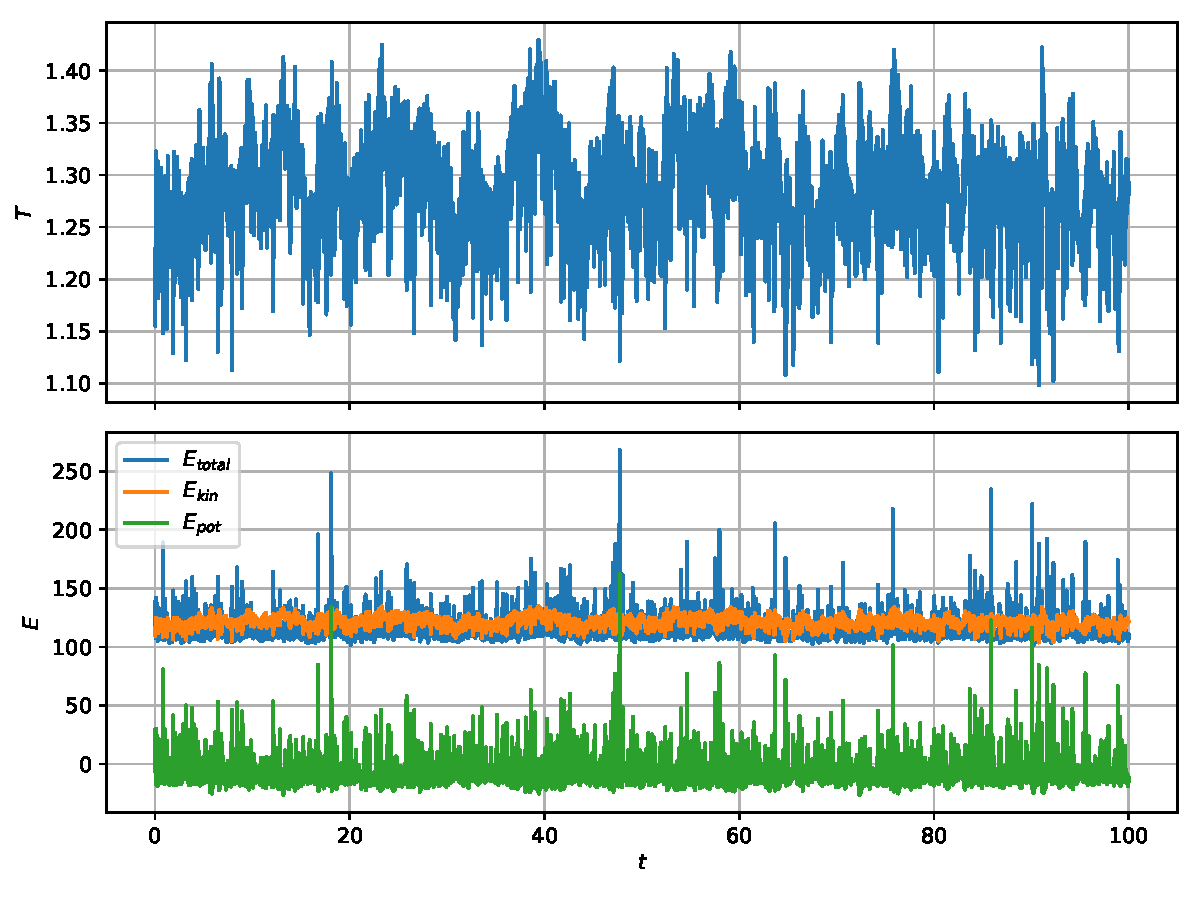
\includegraphics[width=0.8\textwidth]{content/plots/obs_c)_T1.pdf}
    \caption{Energien und Temperatur für $T(0)=1$.}
    \label{fig:obs_1}
\end{figure}
\begin{figure}
    \centering
    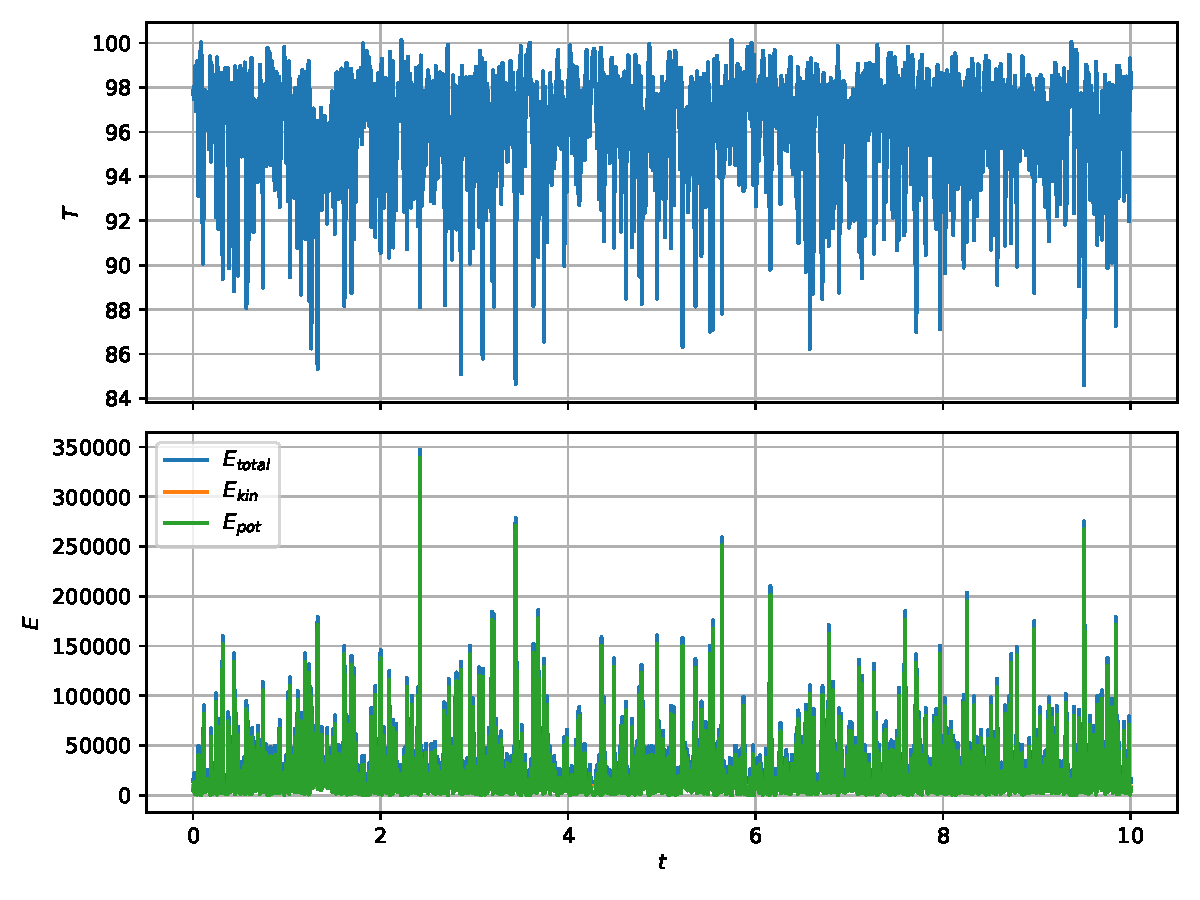
\includegraphics[width=0.8\textwidth]{content/plots/obs_c)_T100.pdf}
    \caption{Energien und Temperatur für $T(0)=100$.}
    \label{fig:obs_100}
\end{figure}

Die Paarkorrelationsfunktion hat bei $T=0.01$ und $T=1$ mehrere Maxima, die mit steigendem $r$ abflachen.
Das System befindet sich in einer flüssigen Phase.
Steigt die Temperatur geht das System in eine gasförmige Phase über.
Dies ist bei $T=100$ der Fall.
Die Paarkorrelationsfunktion weist hier nur ein Maximum auf.
\\
(Leider nicht gut sichtbar, vielleicht besser mit größerem $n$ und $rBins$ aber keine Zeit da kurz vor Abgabe)

\FloatBarrier

\subsection{Isokinetisches Thermostat}
Die Simulation wird nun mit isokinetischem Thermostat durchgeführt.
Dazu wird die Funktion \texttt{IsokinThermostat::rescale} in \texttt{A1.cpp} implementiert, welche die Geschwindigkeiten der Teilchen nach \autoref{eq:isokin} skaliert.
Die Temperatur wird also konstant gehalten.
\\
Es handelt sich um das bereits bekannte Teilchensystem mit Temperatur $T(0)=0.01$.
Zuerst wird die Äquilibrierungsphase mit $\mathrm{d}t=0.01$ und $n=5000$ untersucht.
Die Abbildung \ref{fig:obs_001_iso} zeigt die Energien und Temperaturen in Abhängigkeit der Zeit.
\begin{figure}
    \centering
    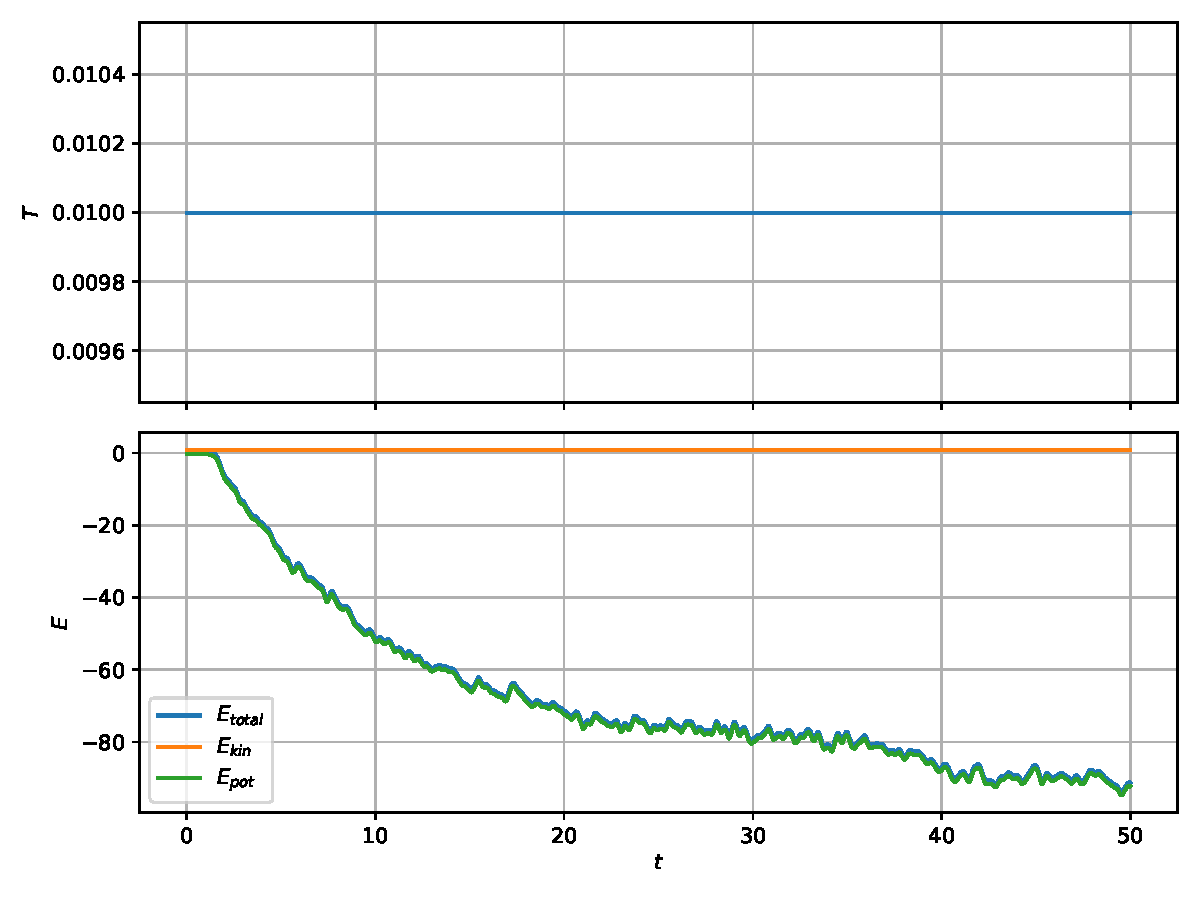
\includegraphics[width=0.8\textwidth]{content/plots/obs_d)_T001_thermo.pdf}
    \caption{Energien und Temperatur für $T(0)=0.01$ mit isokinetischem Thermostat.}
    \label{fig:obs_001_iso}
\end{figure}
Energieerhaltung ist nicht weiter gegeben, da die Temperatur konstant gehalten wird.
Nach etwa $t_\text{equi} \approx 4000$ Schritten konvergiert die potentielle Energie und es stellt sich ein stabiler Zustand ein.
Die Entwicklung des Teilchensystem ist in der Animation \texttt{n8\_T001\_thermo.mp4} für $10000$ Zeitschritte zu sehen.
%Nach etwa $t_\text{equi} \approx 600$ Schritten ist das System äquilibriert.
\\
Es wird nun die Paarverteilungsfunktion mit $n_\text{meas}=10000$ Schritten nach der Äquilibrierungsphase ($n_\text{equi}=5000$) gemessen.
Die Paarkorrelationsfunktion ist in Abbildung \ref{fig:g_001_iso} dargestellt.
\begin{figure}
    \centering
    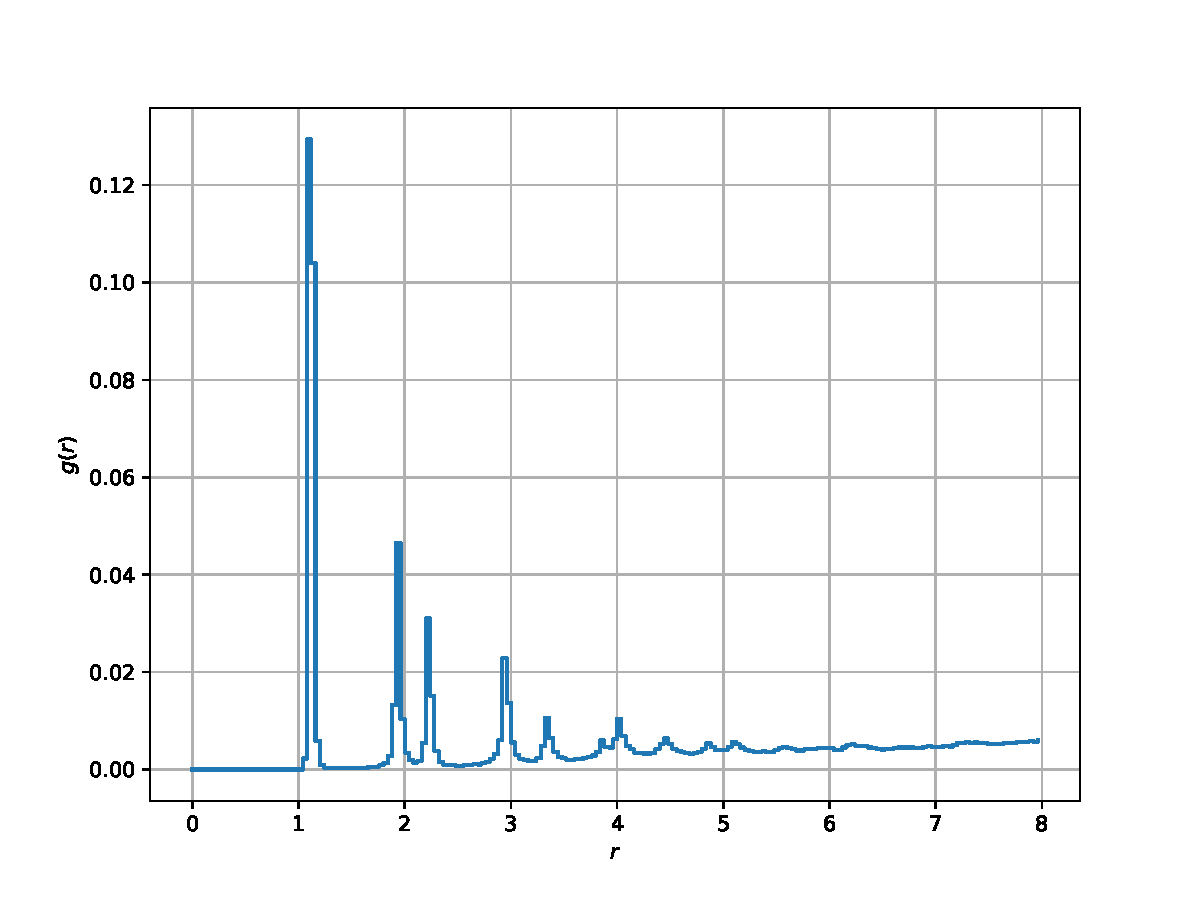
\includegraphics[width=0.8\textwidth]{content/plots/g_d)_T001_thermo.pdf}
    \caption{Paarverteilungsfunktion für $T(0)=0.01$ mit isokinetischem Thermostat.}
    \label{fig:g_001_iso}
\end{figure}

\FloatBarrier
\subsection{Physikalische und chemische Systeme (Kurzfragen)}
\textbf{Which quantities are kept constant during your simulation (after turning on your thermostat)?}
\\
\\
Die Temperatur bzw. die kinetische Energie wird konstant gehalten, die Gesamtenergie ist nicht mehr erhalten.
\\
\\
\\
\textbf{Which thermodynamic ensemble is represented by that?}
\\
\\
Ohne Thermostat: Mikrokanonisches Ensemble ($E$=const.)\\
Mit Thermostat: Kanonisches Ensemble ($T$=const.)
\\
\\
\\
\textbf{You are using an isokinetic thermostat for your system. Is this kind of thermostat physically accurate? If not, name a physically accurate alternative.}
\\
\\
Nein, es ist nicht physikalisch sinnvoll, da die Energien nicht Maxwell-Boltzmann-verteilt sind.
Das Nosé-Hoover Thermostat führt zu Maxwell-Boltzmann-verteilten Energien.
\\
\\
\\
\textbf{A chemist asks you to do a MD-simulation on a chemical solution.
In which way might such a system differ from the ensemble we considered so far?
If you have to keep different quantities constant, name a way to do so for your simulation.}
\\
\\
Unterschiedliche Teilchenarten sind möglich, weitere Wechselwirkungen zwischen Molekülen müssen betrachtet werden.
Weitere Wechselwirkungen können durch zusätzliche Potentiale in der Simulation berücksichtigt werden.
\\
Problematisch wird auch die betrachtete Anzahl der Teilchen in einem chemischen System.
Die Laufzeit für makroskopische Systeme ist zu groß, um sie mit MD zu simulieren.
Coarse-grained Systeme können hier Abhilfe schaffen.
D.h. mehrere Teilchen werden zu einem Teilchen zusammengefasst.
\\
\\
\\
\textbf{Which further potential should also be considered for a chemical solution (f.e. NaCl in water)?}
\\
\\
Das Coulomb-Potential, da es sich um geladene Teilchen handelt.